
One of the fundamental goals for researchers working in the field of artificial intelligence is to make computers act more like ``us''. That is, we can play chess, or drive a car, or control a robot, so why is it so difficult to make a computer program to do things the way \emph{we} do? Unfortunately, human behavior appears to arise from an arcance mix of intuition, acquired knowledge, and calculation. Automated problem solvers have gotten very good at the calculation aspects, but effectively incorporating background knowledge into the agent's calculations remains difficult.

The Bayesian approach to machine-learning attempts to address the knowledge issue. With this approach, knowledge given to the algorithm before any acting occurs or from its own related experiences is formalized into a \emph{prior}. The prior describes what the algorithm designer thinks the world ``might be''. As a result, priors can be either extremely vague or even uninformative, but they can also be exact or nearly exact descriptions of the world. The Bayesian approach to machine-learning takes the prior and combines it with observations made from the world.

In this dissertation, I discuss methods of applying the Bayesian approach to building and using models for sequential decision making. Using a prior to shape an agent's concept of how its environment works can greatly reduce the amount of data it must collect before performing well; if you tell it that something can or can't happen a certain way, it won't need to test those things to find out.

\begin{figure}[t]
\begin{center}
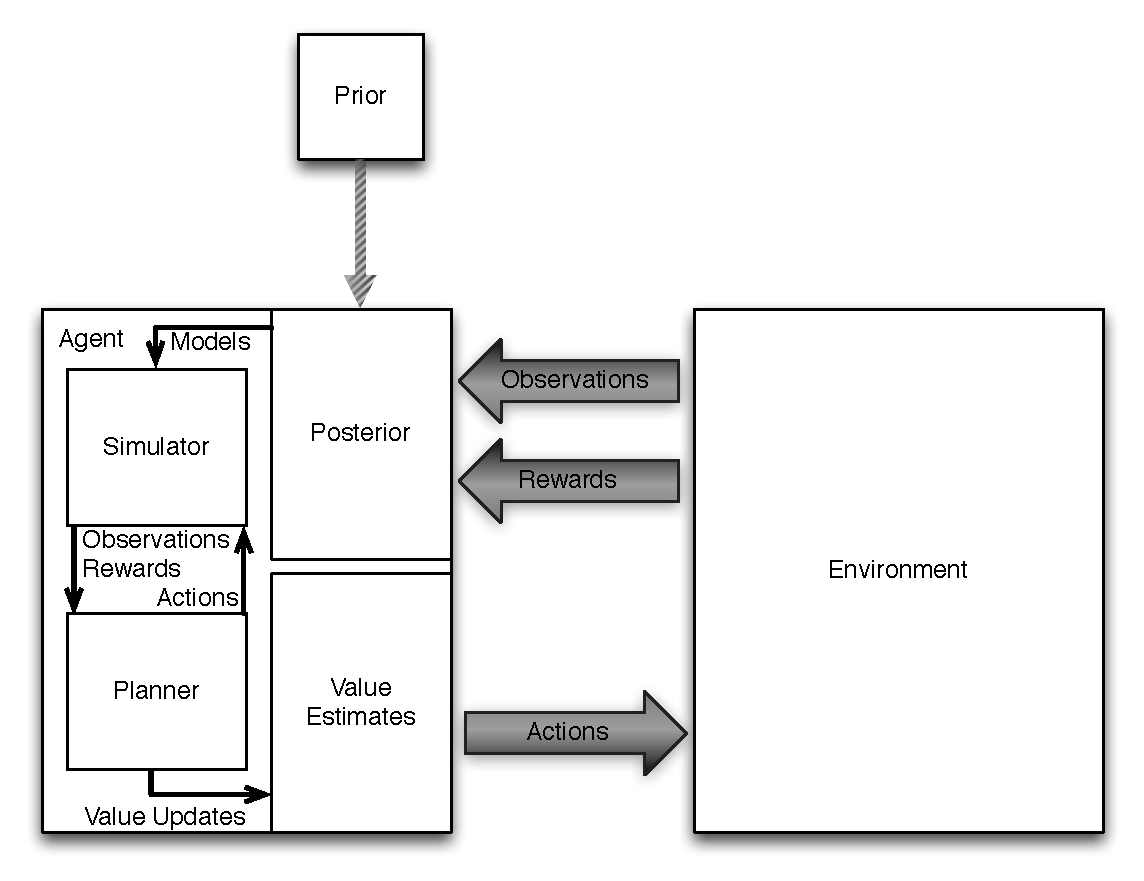
\includegraphics[width=0.49\linewidth]{figures/model_agent.pdf} 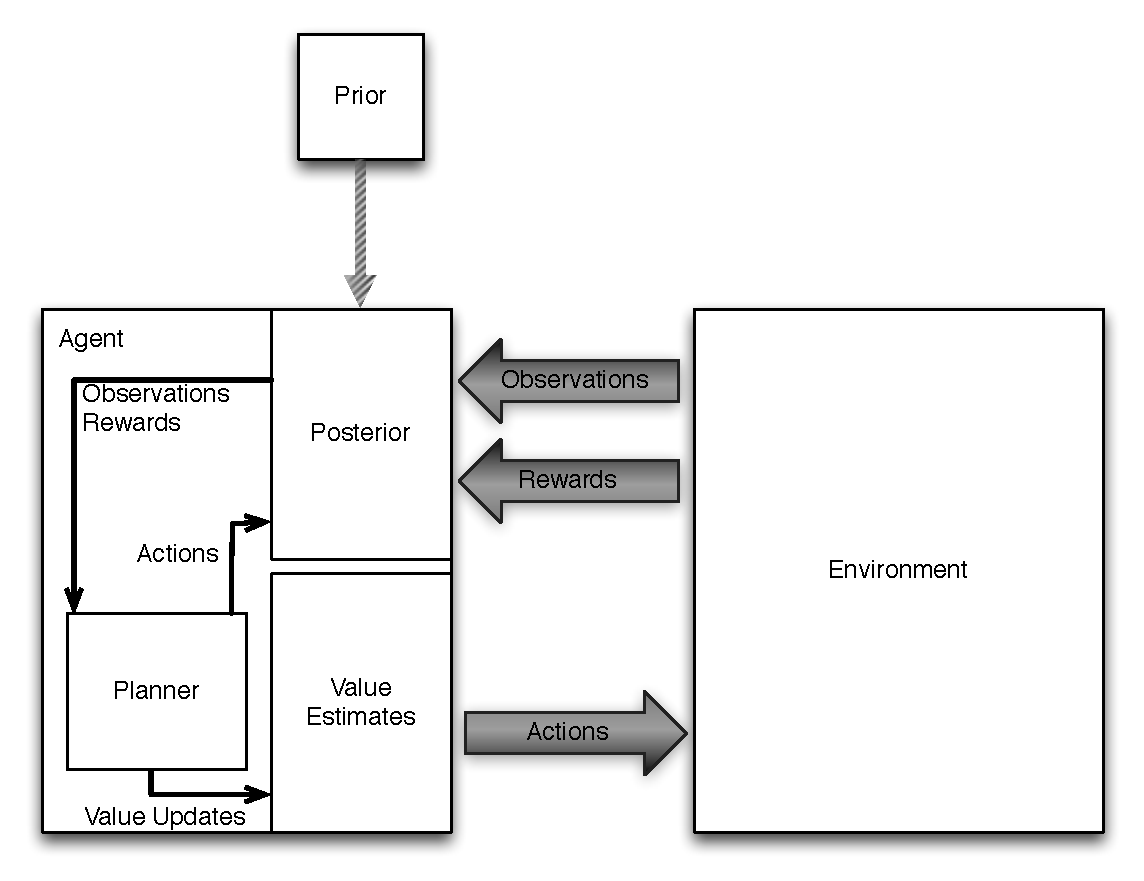
\includegraphics[width=0.49\linewidth]{figures/expr_agent.pdf}
\caption{The two different approaches to Bayesian model-based reinforcement learning that are discussed in this dissertation are the model-sampling approach (left) and the experience-sampling approach (right). With a model-sampling approach, the agent will sample MDPs from the posterior and use those MDPs to run its internal simulation that it uses to create an estimated value function. With an experience-sampling approach, the agent treats the posterior itself as an MDP, and samples observations and rewards directly from the posterior. The two main algorithmic contributions of this dissertation, \alg{BOSS} and \alg{BFS3}, use alternate approaches, with \alg{BOSS} being a model sampler and \alg{BFS3} being an experience sampler.}
\label{sec:intro:agent-blocks}
\end{center}
\end{figure}

The approach I use here to sequential decision making and reinforcement-learning can be divided into distinct blocks: modeling and planning. Figure~\ref{sec:intro:agent-blocks} illustrates the separation of these components. By drawing a strong distinction between the two areas of agent design, one can more easily draw upon the results of their respective communities. The Bayesian machine-learning community focuses its efforts on building complex models that can be used as priors in learning, and works on efficient inference approximations. The planning community focuses its research on efficient ways to act, once given a model. It is only natural to seek to try to turn the fruits of these two communities into a pipeline for learning and sequential decision making.

It is important to note that the best pipeline in this situation is rarely the greedy one, where the agent infers a model, feeds it directly into the planner and follows the planner's advice. In Chapters~\ref{sec:relmbbrl}, \ref{sec:boss}, and \ref{sec:bfs3}, I will describe, motivate and analyze several innovative methods for combining the results of model inference with different sorts of planners.

The particular flavor of learning and sequential decision making problems approached here is called reinforcement-learning. Reinforcement learning provides a flexible way to evaluate a possible behavior through the use of numerical rewards that the agent seeks to maximize. Simple ``find the shortest path to the goal'' behavior, that much of planning research is centered around, is insufficient for many more realistic scenarios where there can be many factors to consider when comparing the ``goodness'' of two agent behaviors.

\section{Reinforcement learning}

Reinforcement learning, or RL, is a framework for problems in which an agent faces both an unknown world and/or an unknown goal. In a reinforcement-learning scenario, the agent interacts with the environment by making observations and performing actions. Each time an action is performed, a new observation is returned to the agent along with a numerical reward signal. The agent's goal is, then, to maximize the cumulative reward over the course of the experiment.

Reinforcement learning model to any problem that has an agent, an environment and rewards. Shortest-path problems can be represented by a reward function that gives $-1$ for each step before the goal, and $0$ or some positive reward for every step after the goal is reached. Bandit problems, a class of reinforcement-learning problems in which the actions taken in the past have no effect on actions taken in the future (though the previous results can affect the agent's \emph{perception} of what might happen in the future), can be mapped to online advertizing, where the agent is trying to figure out what ads a typical user is most likely to click.

The related fields of planning and control theory, while initially appearing to solve many of the same kinds of problems, address only part of the story. Planning and control theory are two ways to figure out what to do in a known-model situation. That is, the situation where you have a complete understanding of the world in which your agent exists, and there is no need to learn about or explore the environment. The field of reinforcement-learning makes the opposite assumption: that some portion of the world must be learned to develop good agent behavior.

With an unknown world, there is a tension between acting to optimize reward based on what the agent already knows, and taking actions that are very likely not the right thing to do, in order to learn more about the world so that the agent can gather reward more efficiently in the future. This tension is referred to as the \emph{exploration/exploitation trade-off}, and is central to the field of reinforcement-learning.

Since the observations made by the agent often correspond strongly with the previous observation and the action performed, reinforcement-learning shares some attributes with active learning. The agent can direct the kinds of data it receives by deciding which action to perform, but it is also limited by the previous observation.

Since it is often difficult to distinguish between two infinite sums, RL researchers lean on the idea of a discount factor, usually labeled $\gamma$. An agent's optimal policy is then the one that maximizes the expected cumulative discounted sum of rewards. This sum is called the expected return. The expected return for a given policy $\pi$ is denoted $R_\pi$:
\begin{eqnarray}
R_\pi &=& \sum_{t=0}^\infty \gamma^t E_\pi[r_t].
\end{eqnarray}
The optimal policy, $\pi^*$, is the policy that maximizes the return:
\begin{eqnarray}
\pi^* &=& \argmax_\pi R_\pi.
\end{eqnarray}


\subsection{Markov Decision Processes}

A common way to concisely describe a reinforcement-learning environment is the Markov Decision Process, or MDP. With an MDP, the observation is a complete description of the configuration, or state, of the world, and the next observed state is a function only of the previous state and action performed. That is, if an agent begins in state $s_1$ and performs action $a_1$, the odds that it ends up in state $s_2$ are the same no matter when this occurs --- the next-state distribution is unchanging. It is important to note that the agent's \emph{impression} of the next-state distribution is free to change, but the actual distribution, which may be unknown, is stationary.

An MDP is formally defined as the tuple $\langle S, A, R, T \rangle$, where $S$ is the set of states, $A$ is the set of actions, $R:S \times A \rightarrow \Re$ is the reward function, and $T:S \times A \rightarrow \Pi(S)$ is the transition function. The state and action sets $S$ and $A$ may be a discrete collection or a continuous range. The reward function $R$ maps state-action pairs to numerical rewards, and the transition $T$ maps state-action pairs to distributions over next-states. Usually, $S$ and $A$ are given, and $R$ and $T$ begin unknown and must be learned.

An MDP is often represented by a graph (for example, see Figure~\ref{intro:mdp}), where nodes are states and edges are actions. At any given time, the agent is said to be \emph{in} some state, and can \emph{take} an action. As a result of taking the action from the state, the agent will receive a numerical reward and end up in another state, or possibly stay in the same state.


\begin{figure}[t]
\begin{center}
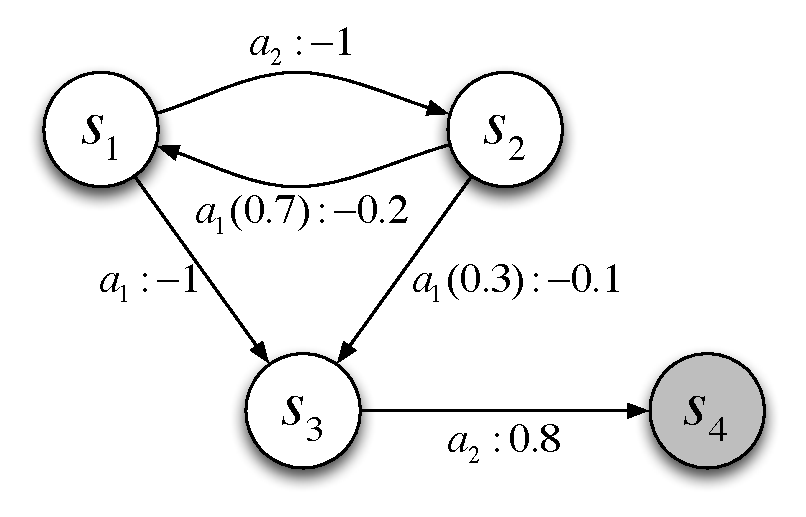
\includegraphics[width=0.5\linewidth]{figures/mdp.pdf}
\caption{an MDP}
\label{intro:mdp}
\end{center}
\end{figure}



The expected return of the optimal policy for the MDP, starting in a particular state, is called the \emph{value} of that state. The value of a state is denoted by $V(s)$, and is captured by a recurrence relation. The expected return for being in a particular state, taking a given action, and following the optimal policy thereafter, is called the \emph{Q-value} of that state-action pair. The Q-value of a state-action pair is denoted by $Q(s,a)$. The functions Q and V can be related by:
\begin{eqnarray}
\label{intro:eqn:value} V(s) &=& \max_a Q(s,a),\\
\label{intro:eqn:qvalue} Q(s,a) &=& R(s,a) + \gamma \sum_{s'} T(s,a)(s') V(s').
\end{eqnarray}
Using the definition of $V(s)$, we know that the optimal policy is the one that always chooses the action with the highest Q-values for the current state.

\subsection{Planning}

The act of finding an optimal or near-optimal policy for a known MDP is called \emph{planning}. Some planning techniques will be given a more thorough treatment in Chapter~\ref{sec:relmbbrl}. This chapter will briefly describe some simple planning techniques.

\subsubsection{Value iteration}

Value iteration, outlined in Algorithm~\ref{alg:vi}, is a planning method which applies the idea of dynamic programming to solving an MDP with a discrete state space and discrete action space. The values that are iterated are the Q-values. The Q-values are given some initial guess (for instance, zero), and Equations~\ref{intro:eqn:value}~and~~\ref{intro:eqn:qvalue} are applied iteratively to all state-action pairs (for the Q-value) and to all states (for the value).

Once the difference between successive estimates of the Q-values, measured by the $\infty$-norm\footnote{The infinity norm of a vector is the absolute value of its largest element.}, is smaller than $(1-\gamma)\epsilon/2$, the difference between the last estimate and the truth is guaranteed to be no larger than $\epsilon$. Eventually, the error will shrink to an acceptably small level, and an approximately optimal policy will be found.

For manageably small numbers of states and actions, value iteration is an effective and easy method for planning. Because the minimum accuracy $\epsilon$ is specified, the algorithm is gauranteed to finish after a finite number of ``sweeps'' of updates over the states.

\begin{algorithm}[tb]
	\caption{$\mbox{Value iteration}(S, A, R, T, \gamma, \epsilon)$}
	\label{alg:vi}
	\KwIn{State set $S$, action set $A$, reward function $R$, transition function $T$, discount factor $\gamma$, accuracy $\epsilon$}
	\KwOut{Q-value table $Q$}
	$\forall_s\ V_0(s)\leftarrow 0$\\
	$\forall_{s,a}\ Q_0(s,a)\leftarrow 0$\\
	$e_0 \leftarrow \infty$\\
	$i \leftarrow 0$\\
	\While {$e_i > \epsilon$} {
		$i \leftarrow i+1$\\
		$e_i \leftarrow 0$\\
		\For {$s \in S$} {
			\For {$a \in A$} {
				$Q_i(s,a) \leftarrow R(s,a) + \gamma \sum_{s'} T(s'|s,a) V_{i-1}(s')$
			}
			$V_i(s) \leftarrow \max_a Q_i(s,a)$\\
			$e_i \leftarrow max(e_i, |V_i(s)-V_{i-1}(s)|)$\\
		}
	}
	\Return $Q_i$
\end{algorithm}

\subsection{Outcomes}

It is often useful to think of transitions from state to state in terms of the \emph{outcome} rather than the resulting state~\cite{jong07,leffler07}.In the context of this dissertation, an outcome is a summary of a change from one state to another. An example in a grid-world is where each state is assigned a coordinate specifying a cell in the grid. With the origin at the bottom left, moving from the cell $(4,2)$ to the cell $(4,3)$ can be described by starting in the cell $(4,2)$ and moving ``up'' $(0,1)$. In this situation, the outcome is ``up'' and it describes how to derive the destination state given the beginning state.

More formally, we have a set of states $S$, a set of outcomes $O$, an outcome function $f:S \times O \rightarrow S$, and an inverse outcome function $f^{-1}: S \times S \rightarrow O$. In the grid-world example, $S$ is the set of all possible cell coordinates, and $O$ is the set $\{\mbox{up},\mbox{down},\mbox{left},\mbox{right},\mbox{stay}\}$. $f$ is a function that takes a state (for instance, $(4,2)$) and an outcome (``up'') and produces the next state ($(4,3)$). The inverse outcome function takes two states and returns the outcome that describes the transition from the first state to the second state if it exists.

The concept of an outcome becomes especially useful when trying to apply the same dynamics to two or more different states. In the grid-world example, it is very likely that every state-action pair has a unique next-state distribution. But, observations on outcomes made in one state can very often be applied successfully to learning another state.

Chapter~\ref{sec:models} discusses some ways in which outcome distributions can be used to cluster states together, and how these groupings can be used to speed learning and drive exploration.

\subsection{Optimality guarantees}

A decision-making algorithm's policy is said to be \emph{optimal} if it maximizes the expected return. Since it is generally impossible to infer an optimal policy before any learning has taken place, weaker guarantees are necessary.

\subsubsection{Convergence}

A reinforcement-learning algorithm has a \emph{convergence guarantee} if it will provably act with the optimal policy in the limit, or after an infinite number of steps in the environment. While this guarantee is fairly weak, theoretically, algorithms that assert it often converge to something near-optimal in a much shorter period of time.

\alg{Q--learning}~\cite{Watkins92} is an example of a reinforcement-learning algorithm with a convergence guarantee.

\subsubsection{PAC-MDP}

\emph{Probably Approximately Correct in MDPs}, or PAC-MDP, is a guarantee that asserts near-optimality with high likelihood in a ``short'' amount of ``time''. An algorithm that is PAC-MDP divides its interactions with the environment into two catagories: exploration steps and exploitation steps. All exploitation steps must have near-optimal actions, or those whose Q--values are within a given accuracy threshold of the state's value, denoted by $\epsilon$. For an algorithm to be PAC-MDP, the number of exploration steps may not exceed a polynomial of the parameters of the environment (often the parameters will be the number of states and actions available in the environment). The algorithm is allowed some overall chance of failure, denoted by $\delta$.

An algorithm that is PAC-MDP will, with high probability, make approximately optimal decisions for all but a polynomial number of steps, where the polynomial is a function of the number of states, actions, $\epsilon$ and $\delta$.

\alg{RMAX}~\cite{brafman02} is an example of a reinforcement-learning algorithm with a PAC-MDP guarantee.


\subsubsection{Bayes-optimal}

\label{sec:intro:bayes-opt}

\emph{Bayes-optimality} is an optimality guarantee made in the context of an MDP prior. The prior distribution acts as knowledge about the environment given to the agent before learning occurs. If the MDP truly is drawn from the provided prior, then the policy that acquires the highest expected return is well-defined, if difficult to compute.

Since every step in the environment affects the agent's belief about the environment in a well-defined way, it is possible to account for all possible step sequences and belief updates over some finite horizon.

\begin{figure}[t]
\begin{center}
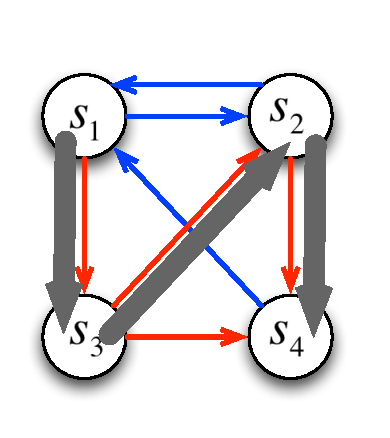
\includegraphics[width=0.25\linewidth]{figures/bamdp-traversal-mdp.pdf}
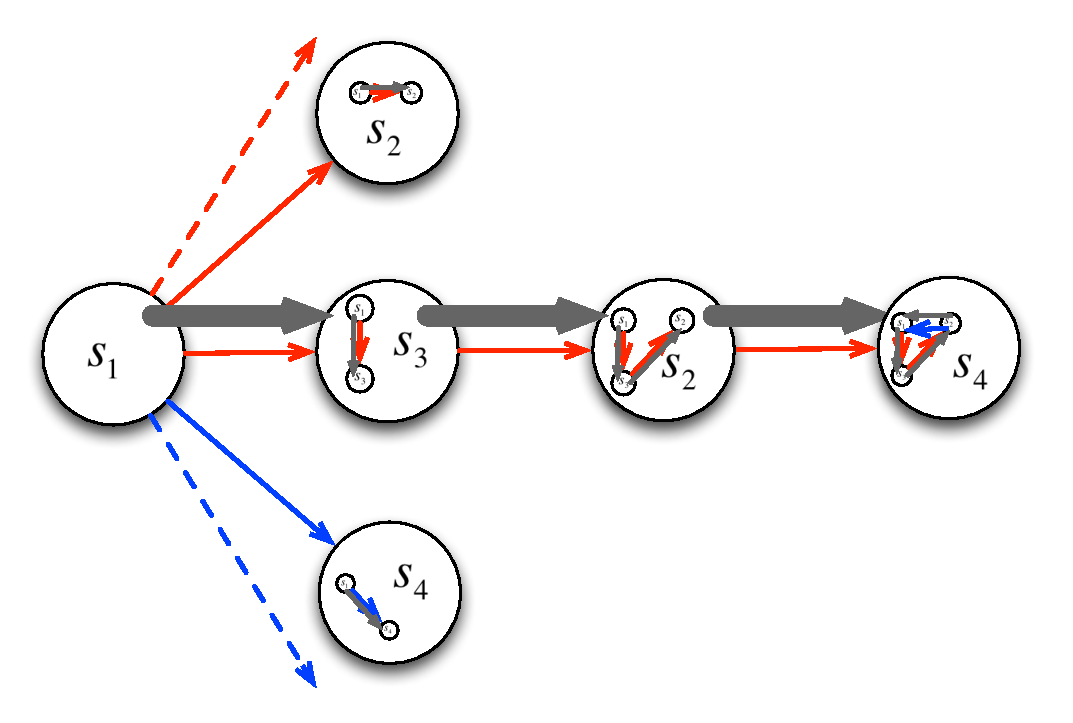
\includegraphics[width=0.55\linewidth]{figures/bamdp-traversal-bamdp.pdf}
\caption{{\bf Left:} an agent makes a trajectory through an MDP, starting at $s_1$ and following the grey arrows.  {\bf Right:} the agent's trajectory through the corresponding BAMDP, where each belief-state has information about what has happened before, as well as the concrete state. Note that once the agent reaches a particular belief-state in the BAMDP, many belief states become unreachable since their internal beliefs are inconsistent with the experience that has been realized.}
\label{intro:bamdp-traversal}
\end{center}
\end{figure}

Bayesian learning in an MDP can be represented by a Bayes-Adaptive MDP, or BAMDP~\cite{duff03}. A BAMDP is a special MDP laid out like a directed acyclic graph whose states are belief-states and whose actions are the actions that can be performed in the actual MDP. The belief-state expresses the agent's knowledge about the environment and a concrete state in which the agent can exist. The knowledge of the environment can be expressed by the combination of the prior and the observations made up to that point, or the posterior.

Figure~\ref{intro:bamdp-traversal} shows a brief MDP traversal and the equivalent traversal in the corresponding BAMDP. Inside each state in the BAMDP, which I will call a \emph{belief-state}, there is a pairing of a \emph{concrete-state} from the real MDP and the history leading to that belief-state. The transition probabilities from belief-states in the BAMDP are known functions of the belief-state's posterior.

The intuition behind the accuracy of the BAMDP for Bayesian-optimal decision making follows. Given some current belief-state for the agent, there is some set of next belief-states that can occur (this set may be infinite or continuous) for each action. The probability of each possible next belief-state is well-defined, and the posterior represented by the belief-state is the combination of the previous posterior and the step that could theoretically have occurred: each of the next belief-states represent one possible world that could result from taking one of the actions.

With a model prior $\phi$ that supports MDPs with state-space $S$, action-space $A$, and discount factor $\gamma$, the corresponding BAMDP is a new MDP with the same action-space and discount factor, but a new state-space. The state-space is $S\times H$, where $H$ is the set of all possible sequences of transitions, where a transition is a tuple $(s, a, s', r)$. The prior $\phi$ can then be conditioned on a history $h$ to get the posterior $\phi|h$. The transition function of the BAMDP $M|\phi$ is then defined to be
\begin{eqnarray}
P(\langle s', h+(s,a,s',r)\rangle|\langle s, h\rangle, a) &=& \int_M P(s', r|s,a,M) \phi(M|h) dM. \label{sec:intro:bamdp-transition}
\end{eqnarray}
In Equation~\ref{sec:intro:bamdp-transition}, the transition likelihood to the concrete state in question, $s'$, is considered for all possible MDPs $M$ and weighted according to their posterior likelihoods, taken from $\phi|h$.

Finding the value of a belief-state can then be done recursively via dynamic programming, treating the set of next belief-states as a set of independent planning problems solved in the exact same way. When the agent takes a step in the actual environment, the agent's new belief matches exactly one of the beliefs considered in the planning problem from the previous state.

If the environment is truly drawn from the agent's prior, simulating experience according to the prior and calculated posteriors is the exact same process as running through a single trajectory in the experiment. In fact, the entire BAMDP is known perfectly. Unfortunately, it is usually difficult to completely solve, since the complete BAMDP has an infinite number of states. Even if we consider only those states reachable in a fixed number of steps (sufficient for approximate planning when there is a discount factor), the number of reachable BAMDP belief-states grows exponentially with that horizon length, the number of actions, and the number of different concrete states reachable in a given transition.

\subsubsection{PAC-BAMDP}

\emph{Probably Approximately Correct for Bayes Adaptive MDPs} (also known as near Bayes-optimal~\cite{kolter09}), or PAC-BAMDP~\cite{araya2012near}, is an optimality guarantee for Bayesian reinforcement-learning.

Exact Bayes-optimal policy inference is generally intractable. Even with a small number of discrete actions and discrete states with a finite horizon, the size of the tree grows exponentially with its depth (with $A$ actions, $S$ states, and a depth of $d$, there can be up to $(A S)^d$ nodes visited by any algorithm. This growth rate means that even if we limit our planning to some depth\footnote{With a discount factor $\gamma$, an accuracy constraint $\epsilon$, and a maximum value $\Vmax$, we need not consider anything farther than $\log_\gamma \frac \epsilon \Vmax$ steps away (see the Bounded Horizon Lemma for details). }, fully evaluating every possibility is very expensive.

As is common in machine-learning tasks, we can opt to satisfy ourselves with a probably approximately correct variation. Instead of considering all possible next belief-states in the search tree, we may consider a sufficiently representative subset. Limiting ourselves to the smaller set introduces some probability of failure, denoted $\delta$. In general, as $\delta$ grows small, the necessary size of the subset grows large. Instead of searching infinitely deep into the tree, we may consider nodes only up to a certain depth. Searching only to some depth introduces an accuracy error, denoted $\epsilon$. In general, as $\epsilon$ goes to zero, the necessary depth of the search tree goes to infinity.

An algorithm that is PAC-BAMDP will, with probability $1-\delta$, make $\epsilon$-Bayes-optimal decisions for all but a polynomial number of steps, where the polynomial is a function of the number of concrete states (not the number of belief-states), actions, $\epsilon$, and $\delta$.

The concept of PAC-BAMDP is not quite on the same level as PAC-MDP. With a PAC-MDP algorithm, it is normally impossible to act optimally for all steps. That is, the polynomial number of mistakes is necessary in order to find the optimal policy later --- there is simply not enough information available to the agent until many potentially sub-optimal steps are taken. With PAC-BAMDP, it is possible to achieve $\epsilon$-$\delta$ Bayes-optimal behavior with \emph{zero} sub-optimal steps. All information needed to act Bayes-optimally is contained in the prior.

An example of an $\epsilon$-$\delta$-Bayes optimal algorithm that requires zero sub-optimal steps is the application of \alg{Sparse Sampling} to the BAMDP. The \alg{Sparse Sampling} algorithm, discussed in detail in Chapter~\ref{sec:relmbbrl}, performs an exhaustive tree search up to some provided depth $d$, trying every action from each visited state $C$ times in order to get a good representation of the next-state distribution. The quantities $d$ and $C$ are chosen to ensure that a $\epsilon$-accurate value for the state is found with probability $1-\delta$. Given $d$ and $C$, \alg{Sparse Sampling} will have to create $(A C)^d$ nodes in its search tree, where $A$ is the number of actions. As a result of this exponential component to the algorithm's runtime, and the fact that $C$ and $d$ need to be phenominally large\footnote{The quantity $C$ must be large enough so that all nodes in the search tree have enough children to be able to estimate their dynamics properly. However, the number of nodes in the search tree grows as a polynomial of $C$. This feedback loop results in bounds for $C$ that are astoundingly high.} to ensure a reasonable accuracy, \alg{Sparse Sampling} is impractical to use even in most trivial problems.

PAC-BAMDP can then be called a compromise between a reinforcement-learning algorithm's sample complexity and computation complexity. \alg{Sparse Sampling} on the BAMDP has a sample complexity of $0$, but an exponential computation complexity. Chapter~\ref{sec:relmbbrl}, on related work, and Chapters~\ref{sec:boss}~and~\ref{sec:bfs3}, on the contributions of this dissertation, describe algorithms with PAC-BAMDP guarantees and several ways to approach the computation complexity issue.

\subsubsection{The PAC-MDP Theorem}
\label{sec:intro:pacmdp-theorem}

This section presents a framework for proving that an algorithm offers a PAC-MDP guarantee.

This proof is an adaptation of earlier work~\cite{lihong09pacmdp,kearns02} with one minor change: instead of saying a particular state-action pair is \emph{known} when it has been tried at least some threshold number of times, a state-action pair is said to be \emph{known} when other state-action pairs of the same \emph{class} have been visited at least some threshold number of times. Introducing the concept of a \emph{class} of state-action pairs allows the analysis to work smoothly with BAMDPs, which have an infinite number of states. Though the number of states may be infinite, we can choose \emph{classes} for each state-action pair that identify what part of that pair is being learned about (that is, we can ignore history when choosing a \emph{class}).

\newtheorem*{horizonlemma}{Bounded Horizon Lemma}
\begin{horizonlemma}
Let $V^\pi_m(s,H)$ be the expected value of following policy $\pi$ in MDP $m$ for $H$ steps, starting at state $s$. Then,
\begin{eqnarray}
V^\pi_m(s,H) &\geq& V^\pi_m(s) - \epsilon_H,
\end{eqnarray}
when
\begin{eqnarray}
H&=&\log_\gamma(\epsilon_H/\Vmax).
\end{eqnarray}

\begin{proof}
Let the return $R$ be the discounted sum of rewards from time-step $0$ onwards, and $R(H)$ be the discounted sum of rewards for the first $H$ steps. That is,
\begin{eqnarray}
R &=& \sum_{t=0}^\infty \gamma^t r_t,\\
R(H) &=& \sum_{t=0}^{H-1} \gamma^t r_t.
\end{eqnarray}
Assuming without loss of generality that $0\leq r_t \leq \Rmax$, we can bound the difference between $R$ and $R(H)$:
\begin{eqnarray}
R - R(H) &=& \sum_{t=H}^\infty \gamma^t r_t,\\
 &\leq& \sum_{t=H}^\infty \gamma^t \Rmax,\\
 &\leq& \frac {\gamma^H} {1-\gamma} \Rmax,\\
 &\leq& \gamma^H \Vmax.
\end{eqnarray}
Therefore, to bound the difference at $\epsilon_H$, we must choose an $H$ such that
\begin{eqnarray}
\epsilon_H &=& \gamma^H \Vmax,\\
H &=& \log_\gamma\left(\frac{\epsilon}{\Vmax}\right).
\end{eqnarray}
If choosing $H$ this way bounds the difference between any sequence of returns and its $H$ horizon to $\epsilon_H$, it must also bound the expected return under any policy.
\end{proof}

%This Lemma is a minor adaptation from previous work~\cite{lihong09horizonlemma} to allow for values bounded by $\Vmax$ instead of values bounded by $1$.

%\label{sec:pacmdp:horizon-error}
%Let $V^\pi_m(s,H)$ be the expected value of following policy $\pi$ in MDP $m$ for $H$ steps, starting at state $s$. Then,
%\begin{eqnarray}
%V^\pi_m(s,H) &\geq& V^\pi_m(s) - \epsilon_H,
%\end{eqnarray}
%when
%\begin{eqnarray}
%H&=&\frac 1 {1-\gamma} \ln\left(\frac \Vmax {\epsilon_H}\right).
%\end{eqnarray}
\end{horizonlemma}

\newtheorem*{simlemma}{Simulation Lemma~\cite{lihong09simlemma,kearns02}}
\begin{simlemma}

\label{sec:pacmdp:simulation}
Let $m_1$ and $m_2$ be two MDPs, such that
\begin{eqnarray}
\forall_{s,a,s'} |T_1(s'|s,a) - T_2(s'|s,a)| &\leq& \epsilon_T,\\
\forall_{s,a} |R_1(s,a) - R_2(s,a)| &\leq& \epsilon_R.
\end{eqnarray}
Then,
\begin{eqnarray}
\forall_s |V_1(s) - V_2(s)| &\leq& s(\epsilon_T,\epsilon_R),\\
\forall_{s,a} |Q_1(s,a) - Q_2(s,a)| &\leq& s(\epsilon_T,\epsilon_R),
\end{eqnarray}
where
\begin{eqnarray}
s(\epsilon_T,\epsilon_R) &=& \frac {\epsilon_R + \gamma \Vmax \epsilon_T} {1-\gamma}.
\end{eqnarray}
\end{simlemma}

\begin{defn}
Let $m$ be an MDP with transition function $T$, reward function $R$, state set $S$ and action set $A$, and let $Q(s,a)$ and $V(s)$ be the $Q$-function and value function for $m$, respectively.
\end{defn}

\begin{defn}
Let $C$ be a set of \emph{classes} for state-action pairs, and let $c:S\times A\rightarrow C$ be a \emph{classifier}. A simple and useful example of a \emph{classifier} would be one that assigns each state-action pair to its own \emph{class}. For a BAMDP, where each BAMDP state is the pairing of a concrete state from the MDP and a history of all transitions observed, the classifier could assign each concrete state and action pair a \emph{class}, ignoring history.
\end{defn}

\begin{defn}
Let $B$ be a knownness threshold. The quantity $B$ needs to be chosen such that if an agent has tried some state-action pair at least $B$ times, it has an approximately accurate estimate of its transition and reward functions.
\end{defn}

\begin{defn}
Let $K_t \subseteq C$ be the set of \emph{known} \emph{classes}, and let $U_t = C - K_t$ be the set of \emph{unknown} \emph{classes}, at time-step $t$. A state-action pair $(s,a)$ is said to be \emph{known} if $c(s,a) \in K_t$.
\end{defn}

\begin{defn}
Let \A be an agent, with
\begin{itemize}
\item
$T_t$ being \As estimate of the transition function at time-step $t$,
\item
$R_t$ being \As estimate of the reward function at time-step $t$,
\item
$Q_t$ being \As estimate of the $Q$-function at time-step $t$,
\item
$\pi_t$ being \As policy at time-step $t$, 
\end{itemize}
such that
\begin{eqnarray}
\pi_t(s_t) &=& \argmax_a Q_t(s_t,a),\\
\forall_{(s,a) | c(s,a)\in K_t} Q_t(s,a) &=& R_t(s,a) + \gamma \sum_{s'} T_t(s'|s,a) V_t(s'),\\
V_t(s) &=& Q_t(s,\pi_t(s)).
\end{eqnarray}
Note that $Q_t(s,a)$ is defined only for \emph{known} state-action pairs. For \emph{unknown} state-action pairs, \A may calculate $Q_t(s,a)$ however it wishes.
\end{defn}

\newtheorem*{pacmdpthm}{PAC-MDP Theorem}
\begin{pacmdpthm}
Let the following conditions be true.
\begin{enumerate}
\item
\label{sec:pacmdp:cond:opt}
Optimism: for any given $c(s,a) \in U_t$, $Q_t(s,a) \geq Q(s,a) - \epsilon_u$.
% with probability at least $1-\delta_u$.
\item
\label{sec:pacmdp:cond:bounded}
Bounded discoveries: if $c(s_t, a_t) \in K_t$, then $\pi_{t+1} = \pi_{t}$,\\ and $\forall_{s,a} \sum_{t=0}^\infty \mathbb{1}\left[(s,a) = (s_t,a_t) \wedge c(s_t,a_t) \in U_t\right] < B$.
\item
\label{sec:pacmdp:cond:acc}
Accuracy: if $c(s,a) \in K_t$, then $\forall_{s'}|T_t(s'|s,a)-T(s'|s,a)| \leq \epsilon_T$ and $|R_t(s,a)-R(s,a)|\leq\epsilon_R$.
% with probability at least $1-\delta_k$.
\end{enumerate}
Then, the expected number of sub-$\epsilon$-optimal actions chosen by agent \A is at most $N = \frac 1 {\delta_l} H B C$, where
\begin{eqnarray}
\delta_l &=& \frac {\epsilon - (\epsilon_u + s(\epsilon_T,\epsilon_R) +2 \epsilon_H)} {\Vmax},\\
s(\epsilon_T,\epsilon_R) &=& \frac {\epsilon_R + \gamma \Vmax \epsilon_T} {1-\gamma},\\
H&=&\log_\gamma\left(\frac {\epsilon_H}{\Vmax}\right),\\
N&\in&\mbox{poly}\left(\frac 1 \epsilon, \Vmax, \frac{1}{1-\gamma},\log\left(\frac {\epsilon_H}{\Vmax}\right), B, C\right).
\end{eqnarray}
\end{pacmdpthm}

\begin{proof}
Lemma~\ref{sec:pacmdp:lemma:opt-steps} shows that if a certain event is sufficiently unlikely during a particular step, that step is $\epsilon$-optimal. Lemma~\ref{sec:pacmdp:lemma:bad-steps} shows that the expected number of steps without that quality is bounded by $\frac 1 \delta_l H B C$.
\end{proof}

\begin{defn}
Let $D_t$ be the event that \A visits an \emph{unknown} state-action pair some time between time-step $t$ and $t+H$. Or, the event $\exists_{0\leq n\leq H} c(s_{t+n},a_{t+n}) \in U_t$.
\end{defn}

\begin{lemma}
\label{sec:pacmdp:lemma:opt-steps}
If $P(D_t) \leq \delta_l$, then $Q(s_t,a_t) \geq V(s_t) - \epsilon$. In other words, if the likelihood of a discovery within $H$ steps is too small, $a_t$ is an $\epsilon$-optimal action in state $s_t$.
\end{lemma}

\begin{proof}

The strategy for this proof is as follows:
\begin{itemize}
\item Speculate the existence of an intermediate MDP $m_t$, which has perfectly accurate dynamics for \emph{known} state-action pairs, and optimistic $Q$-values for \emph{unknown} state-action pairs.
\item Bound the difference between the value of the current policy on the real MDP and on $m_t$.
\item Bound the difference between the value of the current policy on $m_t$ and \As estimate.
\end{itemize}

Let $m_t$ be an MDP with the transition function for any \emph{known} state-action pair (with $c(s,a) \in K_t$) defined to be
\begin{eqnarray}
T_{m_t}(s'|s,a) &=& T(s'|s,a),
\end{eqnarray}
and the $Q$-function for any \emph{unknown} state-action pair (with $c(s,a) \in U_t$) defined to be
\begin{eqnarray}
Q_{m_t}(s,a) &=& Q_t(s,a).
\end{eqnarray}
That is, for \emph{known} state-action pairs, it has the dynamics from the true MDP, and for \emph{unknown} state-action pairs, it uses \As estimate of the $Q$-function.

By applying Condition~\ref{sec:pacmdp:cond:acc} and the simulation lemma, we can bound the difference between its value function and \As estimate:
\begin{eqnarray}
|Q_{m_t}(s,a) - Q_t(s,a)| &\leq& s(\epsilon_T,\epsilon_R),\\
|V_{m_t}(s) - V_t(s)| &\leq& s(\epsilon_T,\epsilon_R),
\end{eqnarray}
where $s(\epsilon_T,\epsilon_R) = \frac{ \epsilon_R + \gamma \Vmax\epsilon_T }{1-\gamma}$.

The value of following policy $\pi_t$ from $s_t$ for $H$ steps in $m$, or $V^{\pi_t}(s_t,H)$, versus the same value in $m_t$, or $V^{\pi_t}_{m_t}(s_t,H)$, can only differ if an \emph{unknown} state-action pair is visited, and then the difference is bounded by $\Vmax$. Therefore,
\begin{eqnarray}
V^{\pi_t}(s_t,H) &\geq& V^{\pi_t}_{m_t}(s_t,H) - \delta_l\Vmax,\\
\label{sec:pacmdp:eqn:extend-horizon}
V^{\pi_t}(s_t) + \epsilon_H  &\geq& V^{\pi_t}_{m_t}(s_t) - \epsilon_H - \delta_l\Vmax,\\
V^{\pi_t}(s_t) &\geq& V^{\pi_t}_{m_t}(s_t) - 2\epsilon_H - \delta_l\Vmax,\\
\label{sec:pacmdp:eqn:apply-sim}
 &\geq& V_t(s_t) - s(\epsilon_T,\epsilon_R) -2 \epsilon_H - \delta_l\Vmax,\\
\label{sec:pacmdp:eqn:get-optimistic}
 &\geq& V(s_t) - \epsilon_u - s(\epsilon_T,\epsilon_R) -2 \epsilon_H - \delta_l\Vmax,\\
Q^{\pi_t}(s_t,a_t) &\geq& V(s_t) - \epsilon_u - s(\epsilon_T,\epsilon_R) -2 \epsilon_H - \delta_l\Vmax,\\
Q(s_t,a_t) &\geq& V(s_t) - \epsilon_u - s(\epsilon_T,\epsilon_R) -2 \epsilon_H - \delta_l\Vmax.
\end{eqnarray}
Equation~\ref{sec:pacmdp:eqn:extend-horizon} is a result of applying the Bounded Horizon Lemma.
Equation~\ref{sec:pacmdp:eqn:apply-sim} is a result of applying the Simulation Lemma.
Equation~\ref{sec:pacmdp:eqn:get-optimistic} is a result of applying the Optimism Condition.


If we choose $\delta_l$ such that
\begin{eqnarray}
\delta_l &=& \frac {\epsilon - (\epsilon_u + s(\epsilon_T,\epsilon_R) +2 \epsilon_H)} {\Vmax},
\end{eqnarray}
then 
\begin{eqnarray}
Q(s_t,a_t) &\geq& V(s_t) - \epsilon.
\end{eqnarray}

\end{proof}

\begin{lemma}
\label{sec:pacmdp:lemma:bad-steps}
The expected number of steps that \A takes where $P(D_t) > \delta_l$ is no more than $\frac 1 {\delta_l} H B C$.
\end{lemma}

\begin{proof}
Let a \emph{discovery} be the event where $c(s_t,a_t) \in U_t$. That is, \A took a step that may change its estimated transition and $Q$-functions.

The number of discoveries is at most $B C$, since each state-action pair's \emph{class} can be visited at most $B$ times before it becomes \emph{known}, and there are $C$ \emph{classes} to choose from.

Let a window of $H$ time-steps beginning at time-step $t$, be called a discovery window if $P(D_t) > \delta_l$, and $t=0$, $P(L_{t-1}) \leq \delta_l$, or $c(s_{t-1},a_{t-1}) \in U_{t-1}$. That is, these windows do not overlap. The probability of a discovery, or visiting an \emph{unknown} state-action pair, is at least $\delta_l$, so the expected number of discoveries per window is at least $\delta_l$.

The expected number of windows per discovery is at most $1/\delta_l$, and since there are $H$ steps per window, the expected number of steps per discovery is $H / \delta_l$.

Since there are at most $B C$ discoveries, the expected number of steps during discovery windows is $\frac 1 {\delta_l} H B C$.

Since any steps taken while not in a discovery window must must be $\epsilon$-optimal, the expected number of sub-optimal steps is at most $\frac 1 {\delta_l} H B C$.
\end{proof}

This proof framework provides a straightforward way to prove that certain classes of reinforcement-learning algorithms have a PAC-MDP guarantee. That is not to say that if an algorithm does not satisfy this framework's conditions, it cannot be PAC-MDP---they are sufficient, but not necessary, conditions.

\section{Bayesian inference}
\label{sec:intro:inf}

Bayesian inference refers to the general technique of combining a prior distribution with observed data to obtain a posterior distribution. Bayesian priors provide principled ways to bring knowledge into a learning problem. The prior distribution encodes the designer's assumption about how the agent's world or environment operates.

Bayesian inference is based on one simple equation, Bayes rule, that relates the prior distribution to the posterior:
\begin{eqnarray}
\label{intro:eqn:bayes} P(H|E) &=& \frac{P(E|H)P(H)}{P(E)},
\end{eqnarray}
where $H$ is the hypothesis and $E$ is the evidence. The quantity $P(H|E)$, or the probability of the hypothesis conditioned on the evidence, is the posterior; $P(E|H)$, or the probability of the evidence conditioned on the hypothesis, is the data likelihood; $P(H)$, or the probability of the hypothesis without regard to the evidence, is the prior; $P(E)$, or the probability of the evidence without regard to the hypothesis, plays the role of a normalizing factor and is not calculated directly.

\subsection{Coin flipping}
\label{sec:intro:coin-flipping}
An example that can illustrate the Bayesian inference process is that of learning the bias of a coin by flipping it a number of times.

Suppose there is a bag of $10000$ coins, $10$ of which are two-headed. The remaining $9990$ coins are fair coins, equally likely to flip heads or tails. The experiment is to take a coin from this bag, and track how likely it is that the coin is biased after some number of $n$ observed flips.

First, there must be a generative model to describe the experiment dynamics:

\begin{eqnarray}
\label{intro:eqn:coinbag}\rho &\sim&
\left\{\begin{array}{lll}
0.5 & \mbox{w.p.} & 9990/10000,\\
1 & \mbox{w.p.} & 10/10000,
\end{array}\right.\\
\label{}H &\sim& \mbox{Binomial}(\rho, n),
\end{eqnarray}
where $\rho$ is the bias of the coin, either $0.5$ (fair) or $1$ (two-headed), $n$ is the number of flips made, and $H$ is the number of flips observed to be heads.

The number of observed heads, $H$, is drawn from the binomial distribution, which has the probability mass function 
\begin{eqnarray}
\label{intro:eqn:binomial} P(H=h|\rho, n) = {n \choose h} h^\rho (n-h)^{1-\rho}.
\end{eqnarray}

The prior distribution of the coin's bias is defined explicitly in the generative model, in Equation~\ref{intro:eqn:coinbag}. To find the corresponding posterior distribution, one must use Bayes rule from Equation~\ref{intro:eqn:bayes}.

The posterior, $P(\rho|h,n)$, can be formulated by applying Bayes rule.

\begin{eqnarray}
P(\rho|h,n) & \propto & P(h|\rho,n)P(\rho|n),\\
\label{intro:eqn:coinprop} & \propto & P(h|\rho,n)P(\rho)\\
&\propto& {n \choose h} h^\rho (n-h)^{1-\rho} P(\rho)\\
&\propto& h^\rho (n-h)^{1-\rho} P(\rho).
\end{eqnarray}

From our original model, Equation~\ref{intro:eqn:coinbag} tells us that there are only two possibilities for $\rho$: $0$ or $0.5$. To find their exact posterior likelihoods, we can evaluate Equation~\ref{intro:eqn:coinprop} for both and normalize.

\begin{eqnarray}
P(\rho=0.5|H=h,n) & \propto & {0.5}^h {0.5}^{n-h} \cdot \frac{9990}{10000}\\
& \propto & {0.5}^n \cdot \frac{9990}{10000}.
\end{eqnarray}

\begin{eqnarray}
P(\rho=1|H=h,n) & \propto &  1^h 0^{n-h} \cdot \frac{10}{10000}.
\end{eqnarray}

Let's first evaluate the posterior likelihood that $\rho=1$.
\begin{eqnarray}
\label{intro:eqn:coin-post}P(\rho=1|H=h,n) & = & \frac{1^h 0^{n-h} \cdot \frac{10}{10000}}{1^h 0^{n-h} \cdot \frac{10}{10000}+{0.5}^n \cdot \frac{9990}{10000}}.
\end{eqnarray}

There are two basic cases:
\begin{enumerate}
\item \label{intro:eqn:case-allheads} Every flip was heads, or $h=n$.
\item \label{intro:eqn:case-notallheads} Not every flip was heads, or $h<n$.
\end{enumerate}

In Case~\ref{intro:eqn:case-allheads}, when $h=n$, Equation~\ref{intro:eqn:coin-post} can be used to evaluate the posterior exactly.

In Case~\ref{intro:eqn:case-notallheads}, when $h<n$, $P(\rho=1|H=h,n)$ goes to zero because of the $0^{n-h}$ term in the numerator.

This same process, applying Bayes rule to turn a prior and observations into a posterior, is the basis for all models discussed in this work.

\subsection{The Chinese Restaurant Process}

The Chinese Restaurant Process, or CRP, is a nonparametric prior that can be used to guess assignments of elements in a set to clusters~\cite{teh2010dirichlet}. Here, the word nonparametric indicates that the number of parameters supplied by the CRP posterior is not known in advance and instead depends on the size of the observation set that it is given.

\begin{figure}[t]
\begin{center}
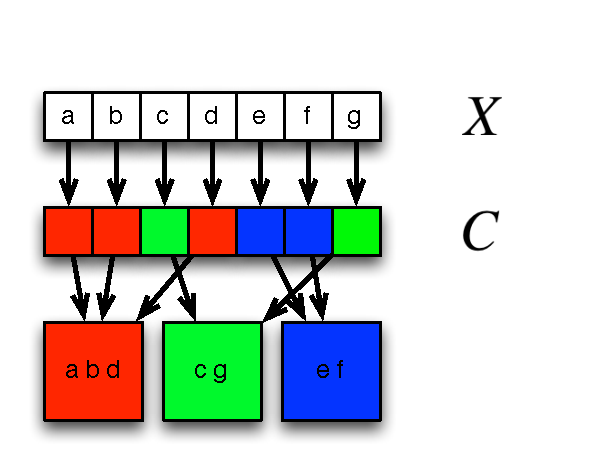
\includegraphics[width=0.4\linewidth]{figures/crp-mixture.pdf}
\caption{}
\label{intro:crp-mixture}
\end{center}
\end{figure}


The CRP prior likelihood is easy to evaluate online. For a new element, the prior likelihood that it belongs to any given cluster is proportional to the number of elements already in that cluster, and the prior likelihood that it belongs in a new cluster is proportional to a parameter $\alpha$.

Inference on mixture models can often be done with a CRP. A generative mixture model follows. The observed data $X$ and the base measure $G_0$ are given, and $\alpha$ is a parameter that influences cluster size:

\begin{eqnarray}
F_i&\sim&G_0\\
C&\sim&CRP(\alpha)\\
X_t&\sim&F_{C_t}.
\end{eqnarray}
Here, $C$ is a vector and $C_t$ is the index of the cluster assigned to the data point $X_t$. $F_i$ is the sampling distribution associated with cluster $i$, and is drawn from the base measure $G_0$. Figure~\ref{intro:crp-mixture} illustrates how the data in $X$ is clustered by $C$, the assignment from the CRP.

The task here is to perform inference on the assignments $C$ and the cluster distributions $F_i$. It is useful to choose cluster distributions $F$ and base measure $G_0$ such that $G_0$ is conjugate prior to $F$. Conjugacy allows us to easily derive a posterior $F~\sim~G_0|D$ and to calculate the ``clustering likelihood'' $P(X|C,G_0)=\prod_i\int_{F_i} F_i(X^i)G_0(F_i)dF_i$ analytically, where $X^i=\{X_t|C_t=i\}$ is the collection of data from $X$ assigned to cluster $i$. 

The conjugacy between $F_i$ and $G_0$ allows us to sample the assignment vector $C$ with no knowledge of the parameters for $F_i$. $C$ is sampled from the distribution $P(C|X,G_0,\alpha)\propto P(X|C,G_0)P(C|\alpha)$. This step in itself is useful, as clustering has been performed. If more data needs to be generated for simulation, a new point $X_j$'s cluster can be chosen according to $P(C_j|C_{-j},\alpha)$, that cluster's distribution $F_{C_j}$ can be chosen from $G_0(F_{C_j}|X^{C_j})$ and $X_j$'s value can be chosen according to $F_{C_j}(X_j)$.

There is also a closed form for the CRP prior, $P(C|\alpha)$:
\begin{eqnarray}
P(C|\alpha)&=&\alpha^r \frac {\Gamma(\alpha)}{\Gamma(\alpha+\sum_i n_i)}\prod_i\Gamma(n_i),\label{eq:crp}
\end{eqnarray}
where $n_i = \sum_{j} \delta_{C_j,i}$, and $\delta_{i,j}=1$ iff $i=j$, is the number of elements assigned to cluster $i$, and $r$ is the number of clusters with at least $1$ member.

The CRP is exchangeable. That is, the order of the elements does not affect the posterior assignment distribution.

It is worth noting that the number of possible vectors $C$ grows exponentially with the number of elements in $X$. For CRP inference, Gibbs sampling~\cite{andrieu03,neal00} is a practical way to do approximation.

\section{Bayesian models for reinforcement-learning}
\label{sec:intro:rl-models}

As mentioned briefly at the beginning of this chapter, the Bayesian approach to learning can be applied to modeling reinforcement-learning domains. There exist Bayesian approaches to model-free reinforcement-learning~\cite{dearden98}, but they do not fit within the scope of this dissertation devoted to model-based reinforcement-learning.

For model building for reinforcement-learning, we must first start with a model prior. We combine it with observations made by the agent to derive a model posterior. This model posterior can be used for reasoning about future choices that the agent will make.

\subsection{Flat Dirichlet multinomial}

\label{intro:fdm}

For a discrete-state -action MDP, the \prior{Flat Dirichlet Multinomial}, or \prior{FDM}, prior can be used~\cite{poupart06}. According to the \prior{FDM} prior, the next-state distributions for all state-action pairs are multinomials whose parameters are drawn i.i.d. \ from the Dirichlet distribution, parameterized by some constant vector $\alpha$:
\begin{eqnarray}
\theta^{s,a} &\sim& \mbox{Dirichlet}(\alpha),\\
N^{s,a} &\sim& \mbox{Multinomial}(\theta^{s,a}).
\end{eqnarray}

Because the Dirichlet distribution is conjugate to the multinomial distribution, the \prior{FDM} posterior is easy to compute:
\begin{eqnarray}
\label{intro:eqn:fdm-theta}\theta^{s,a}|N^{s,a} &\sim& \mbox{Dirichlet}(\alpha+N^{s,a}),\\
\label{intro:eqn:fdm-s}P(s'|N^{s,a},\alpha) &\propto& \alpha_{s'}+N^{s,a}_{s'}.
\end{eqnarray}

The derivation for Equations~\ref{intro:eqn:fdm-theta}~and~\ref{intro:eqn:fdm-s} are a result of Equation~\ref{sec:models:dir-mult-conj} in Chapter~\ref{sec:models}.

Equation~\ref{intro:eqn:fdm-theta} gives us the ability to sample from the MDP posterior. Equation~\ref{intro:eqn:fdm-s} gives us the ability to sample experience, and as a result \prior{FDM} can be considered a trajectory prior. This capability is useful if the planner wants only a simulation oracle, and doesn't care about entire models.

This prior is theoretically attractive, since it easily supports all possible discrete-state discrete-action MDPs. but not good at generalizing as it treats estimating each state-action as a separate learning problem. On the other hand, a different choice of the $\alpha$ parameter for each state-action pair can be used to essentially \emph{know} the MDP before hand - with some uncertainty built in where appropriate. RL agents that rely on the \prior{FDM} prior generally are unlikely outperform non-Bayesian agents; if the prior knowledge states, essentially, that it is an MDP and the transition functions can be any multinomial, this information does not give the Bayesian agent a leg up on other agents, since this assumption will usually be baked into the algorithm design from the beginning.

\subsection{Gaussian bandits}

For a bandit problem in which the reward for an arm can be any real number, the \prior{Gaussian bandit} prior can be used~\cite{wang05}:
\begin{eqnarray}
\label{intro:eqn:gband-mu}\mu^a &\sim& N(\mu_0, \sigma^2_0),\\
\label{intro:eqn:gband-r}R_t^a &\sim& N(\mu^a, \sigma^2).
\end{eqnarray}

In Equations~\ref{intro:eqn:gband-mu}~and~\ref{intro:eqn:gband-r}, $\mu_0$ and $\sigma_0$ are parameters indicating where the reward averages are likely to be, and $\sigma$ is a parameter indicating the variance in the reward seen for a particular arm. The value $\mu^a$ is the expected reward acquired from pulling arm $a$, and $R_t^a$ is the reward acquired from pulling arm $a$ for the $t^{\mbox{th}}$ time.

Like the \prior{FDM} prior in Section~\ref{intro:fdm}, the \prior{Gaussian bandit} prior makes use of conjugacy for efficient inference. The known-variance Normal distribution is its own conjugate prior:
\begin{eqnarray}
\label{intro:eqn:gband-post}\mu^a|R^a &\sim& N\left(\left(\frac{\mu_0}{\sigma_0^2} + \frac{\sum_{t=1}^T R_t^a}{\sigma^2}\right)/\left(\frac 1 {\sigma_0^2} + \frac T {\sigma^2} \right), \left(\frac 1 {\sigma_0^2} + \frac T {\sigma^2} \right)^{-1}\right).
\end{eqnarray}

While the \prior{Gaussian bandit} prior does not model all possible continuous-reward distributions like the \prior{FDM} prior models all possible discrete MDPs, it can still be used to trade-off uncertainty in the mean (indicated by the $\sigma_0^2$ parameter) and knowledge of the mean gathered from data, expressed in Equation~\ref{intro:eqn:gband-post}.

\section{Model-based Bayesian reinforcement learning}

This dissertation focuses on developing models appropriate to reinforcement-learning domains, the algorithms that can take advantage of these models to effectively solve the reinforcement-learning problem, and the analysis of these algorithms.

Chapter~\ref{sec:models} will extend the ideas from Section~\ref{sec:intro:inf} and Section~\ref{sec:intro:rl-models} to create more structured and useful models.

Chapter~\ref{sec:relmbbrl} is a survey of existing model-based and Bayesian model-based reinforcement-learning algorithms.

Chapter~\ref{sec:boss} introduces the \alg{Best Of Sampled Set} algorithm and its analysis.

Chapter~\ref{sec:bfs3} introduces the \alg{Bayesian Forward Search Sparse Sampling} algorithm and its analysis.

Chapter~\ref{sec:experiments} reports on several experimental results comparing Bayesian model-based reinforcement-learning algorithms against each other and other model-based reinforcement-learning algorithms.

Chapter~\ref{sec:conclusion} concludes the dissertation and summarizes its contributions.

%
\ifperchapterbib%
For the convenience of the reader, a list of references is provided at the end of each chapter (where applicable).
\ifendbib%
A bibliography containing all cited references is included at the \hyperref[sec:bibliography]{end of the dissertation}.
\else\fi% end ifendbib
\cbend%
\else\fi% end ifperchapterbib